Based on the abstract system structure as presented in chapter \ref{chp:structure} a platform specific software structure needs to be defined for the Android OS platform.This structure is shown in figure \ref{android_structure}. It respects Android specific constructs, patterns and object-types.\\\\
\begin{figure}[h!]
\centering
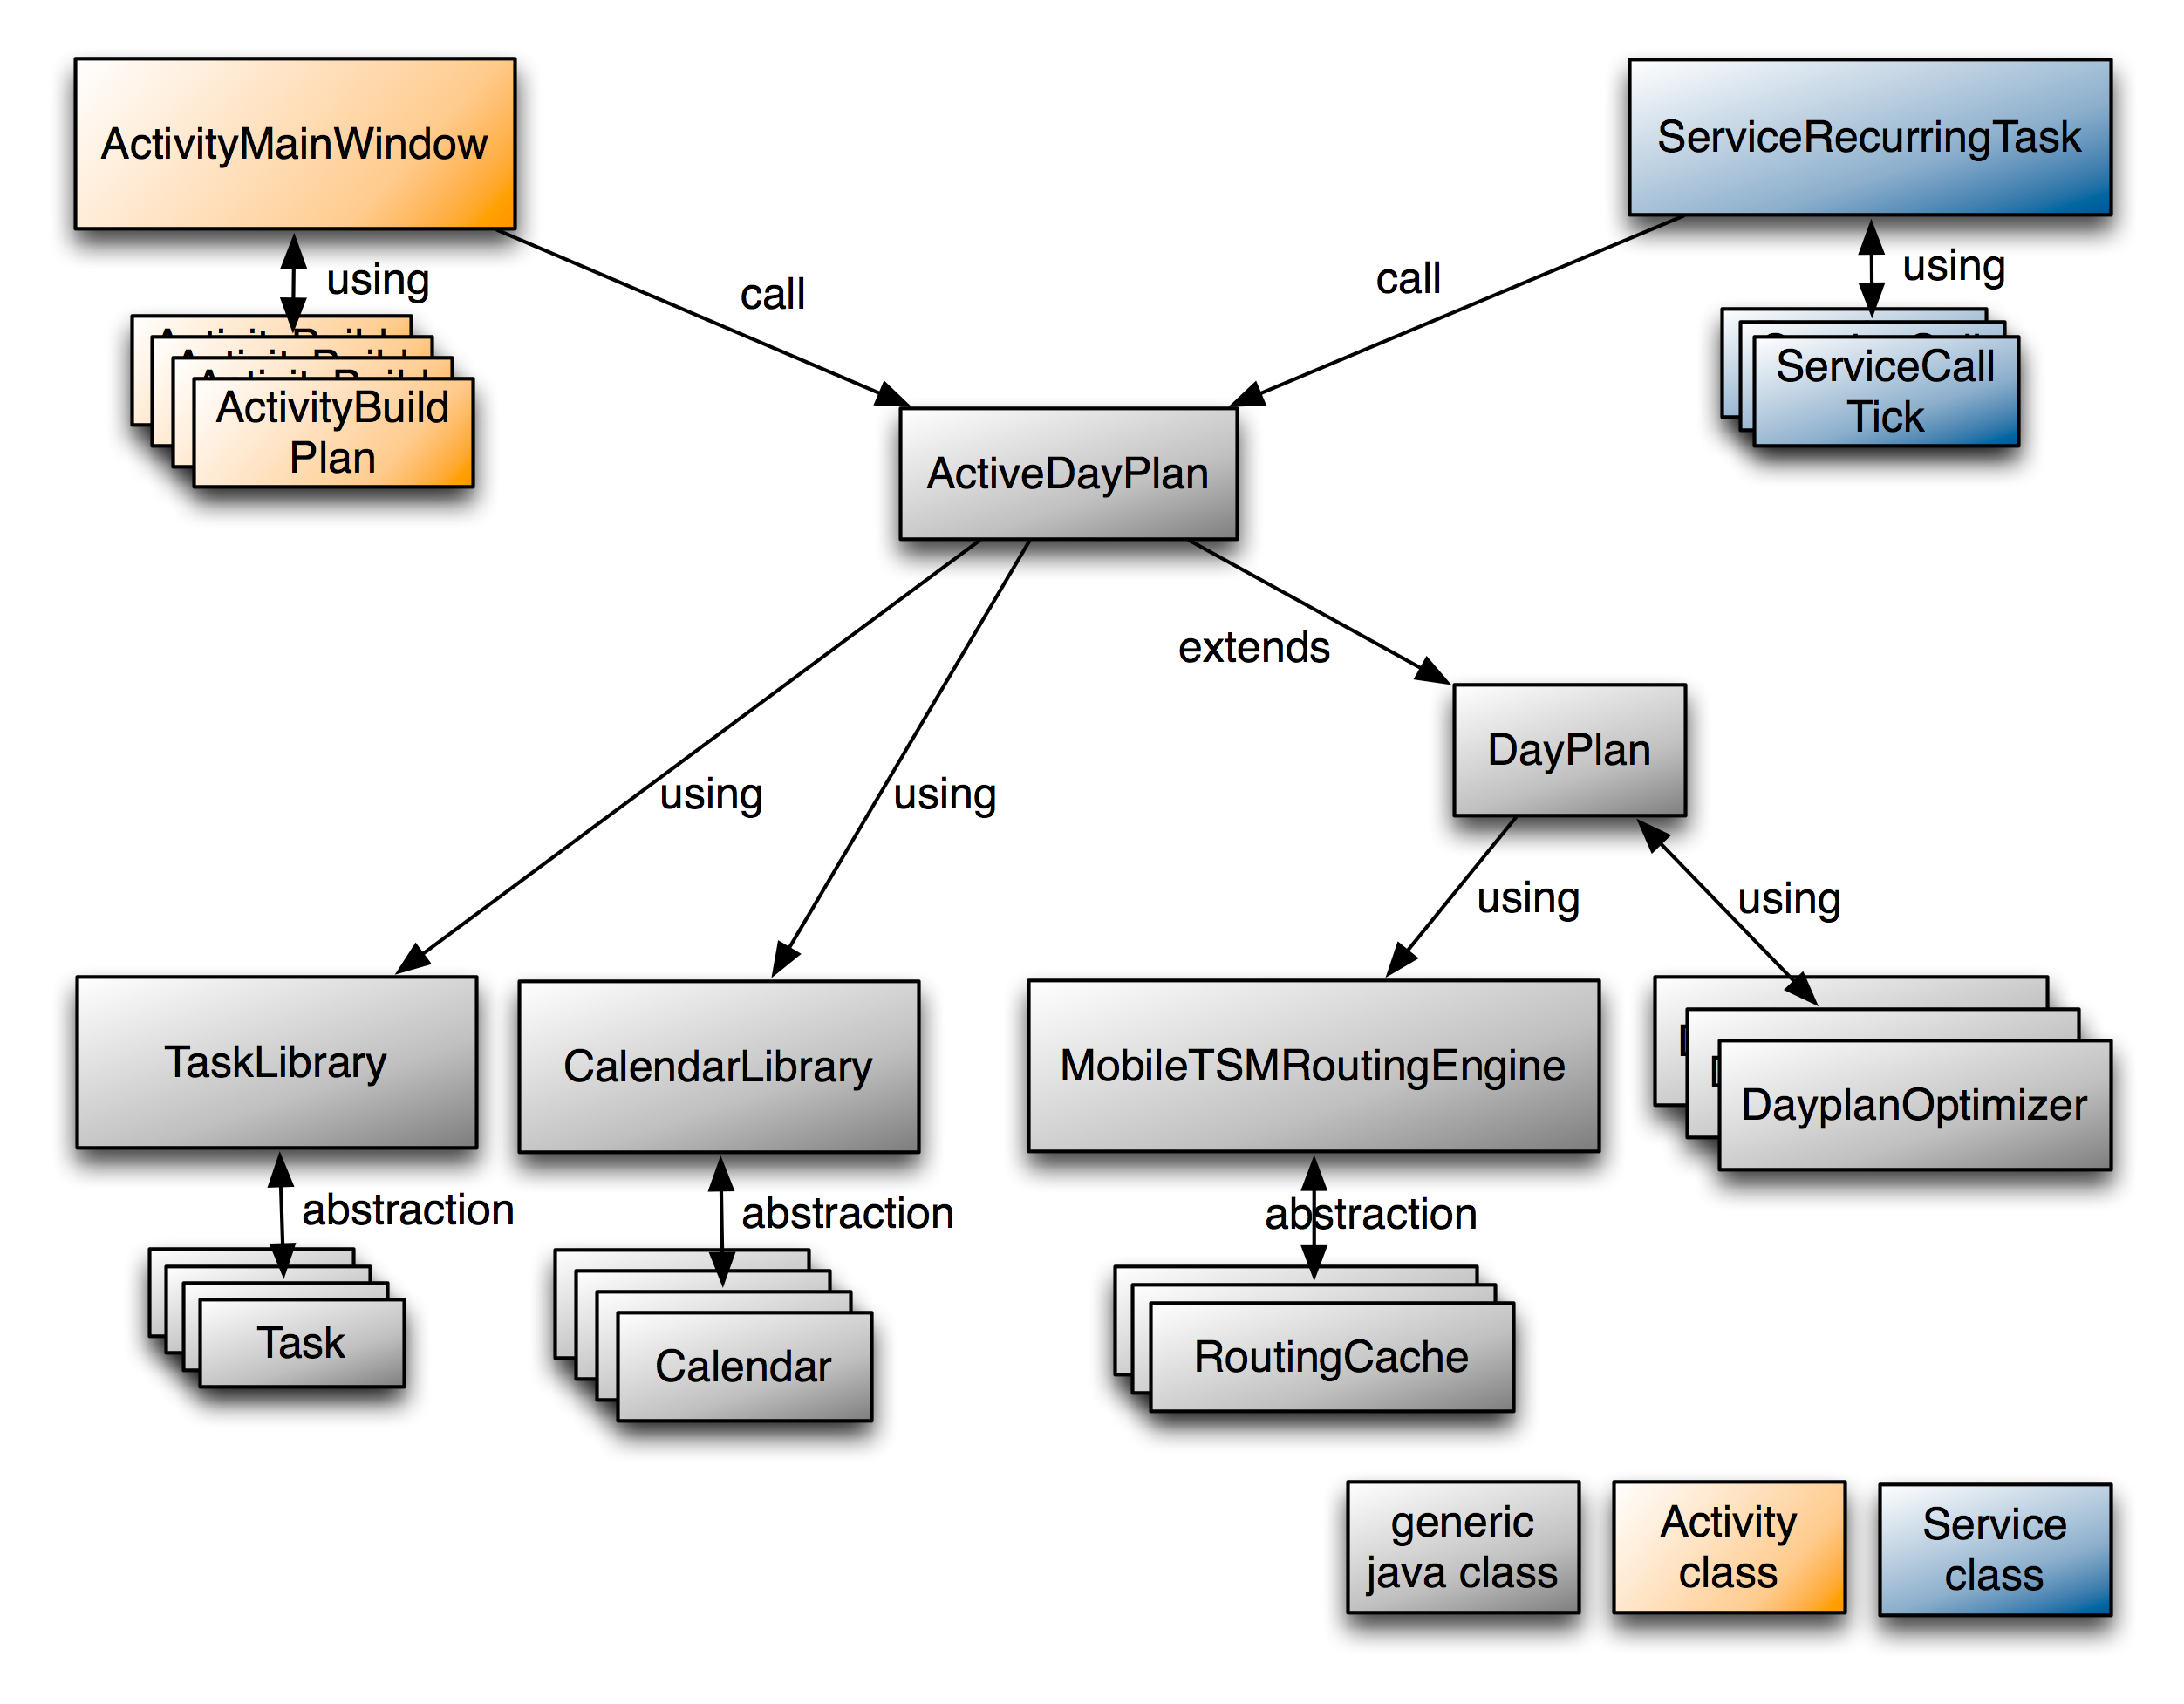
\includegraphics[width=14cm]{pics/android_structure.png}
\caption{Platform specific software structure for Android OS}
\label{android_structure}
\end{figure}
The classes marked in orange extend the platform specific Activity-class. In Android OS, Activities are used to build the graphical user interface (GUI). The class ActivityMainWindow contains a tabbing element, the other Activities from the com.kangaroo.gui package are wrapped in the individual tabs. A detailed description of the Kangaroo GUI can be found in chapter \ref{sec:user_interface}\\\\
The blue classes extend the Service-class. In Android OS Services are used to execute computations that are independent of the user interface.  The ServiceRecurringTask class in com.kangaroo.system implements a background task that is executed over and over independently of user interaction. The other Services shown here are helper classes that make sure the background task is called when the location of the device in time or space has changed. These system integration classes are explained in the chapter \ref{sec:android_integration} \\\\
All classes kept in grey are generic java classes. These system elements do not directly extend the Android platform, although some of them might use platform specific data types and methods. The classes can be divided into the following groups:
\begin{itemize}
\item TaskLibrary: The TaskLibrary and other related classes in the package com.kangaroo.task provide the functionality to store and manage tasks. These classes are described in chapter \ref{sec:android_task} 
\item CalendarLibrary: The classes in com.kangaroo.calendar provide a wrapper for the non public Android calendar API. A description of the classes and the reverse-engineering process can be found in chapter \ref{sec:android_calendar}.
\item MobileTSMRoutingEngine and the other classes in the com.mobiletsm.* package provide routing functionality for Kangaroo. The routing is described in chapter \ref{sub:routing}
\item DayPlan: The DayPlan and related classes in com.kanaroo implement temporal storage of events and tasks. Also these classes provide the functionality for checking and optimizing of the day plans. These classes can be found in chapter \ref{sub:dayplan} 
\end{itemize}
